\section{Definition, Classification and Properties of Signals}
\subsection{Definition of signals}
 \begin{itemize}
    \item  Signals describe physical phenomena as patterns of variations of some form.
    
    \item Mathematically, signals are \textbf{functions} of one or more independent variables.
    
    \item For example, a signal $s(t)$ can be a function of the continuous independent variable time $t \in [\alpha, \beta]$ A two-dimensional signal $f(x, y)$ can be a function of two spatial coordinates $x, y$.
 \end{itemize}

\subsection{Continuous and Discrete-time Signals}
 \begin{itemize}
    \item Signals can be a function of the \textbf{continuous time} variable, in which case we will use the notation $x(t)$ with $t \in \mathbb{R}$, \\
    or of the \textbf{discrete time} variable, in which case we will use the notation $x[n]$ with $n \in \mathbb{Z}$. (\textsc{Fig.1})

 
 \begin{figure}[H]
 \begin{minipage}{0.5\textwidth}
  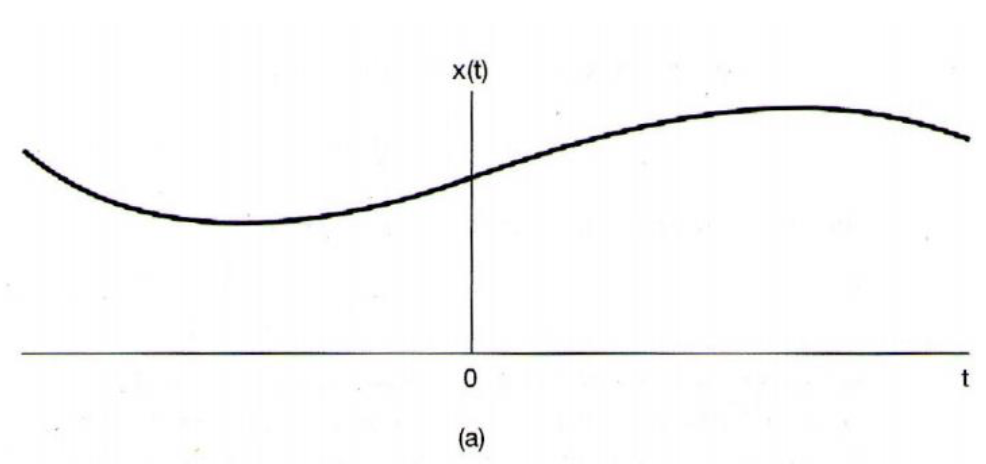
\includegraphics[width = \textwidth]{images/continuous_signals}
  \end{minipage} \hfill
  \begin{minipage}{0.5\textwidth}
  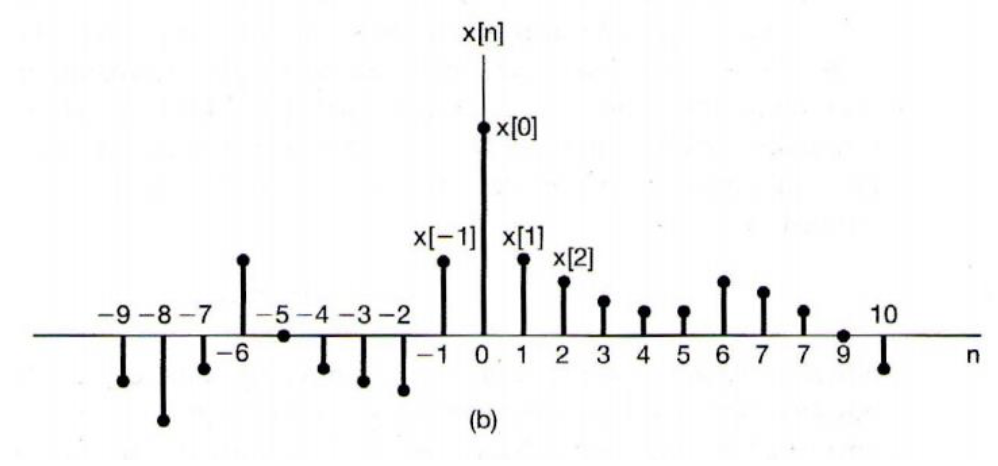
\includegraphics[width=\textwidth]{images/discrete_signals}
  \end{minipage}
  \caption{Continuous signal $x(t)$ and discrete signal $x[n]$ }
 \end{figure}
 
    \item Discrete-time signals are often (but not necessarily) a sampling of continuous-time signals.
    \[ x[n] = x_{c}(nT) \quad -\infty < n < +\infty \]\ $T$ is sampling period.
 
    \item A discrete-time signal can be represented as a sequence of numbers, or, a vector.
 \end{itemize}

 \subsubsection{Digital Signals}
 \begin{itemize}
    \item When we speak of a digital signal we often mean one that has been \textbf{sampled} (captured at regular points in time) and \textbf{quantisised}.
    
    \item When one refers to a 12-bit signal, they are referring to the number of amplitude quantisation levels.
    
    \item Sampling a continuous signal may be done \textbf{without losing any information} from the original signal. Conversely, quantisation always implies \textbf{losing information}. (\textsc{Fig.2})
 \end{itemize}
 \begin{figure}[h!]\centering
    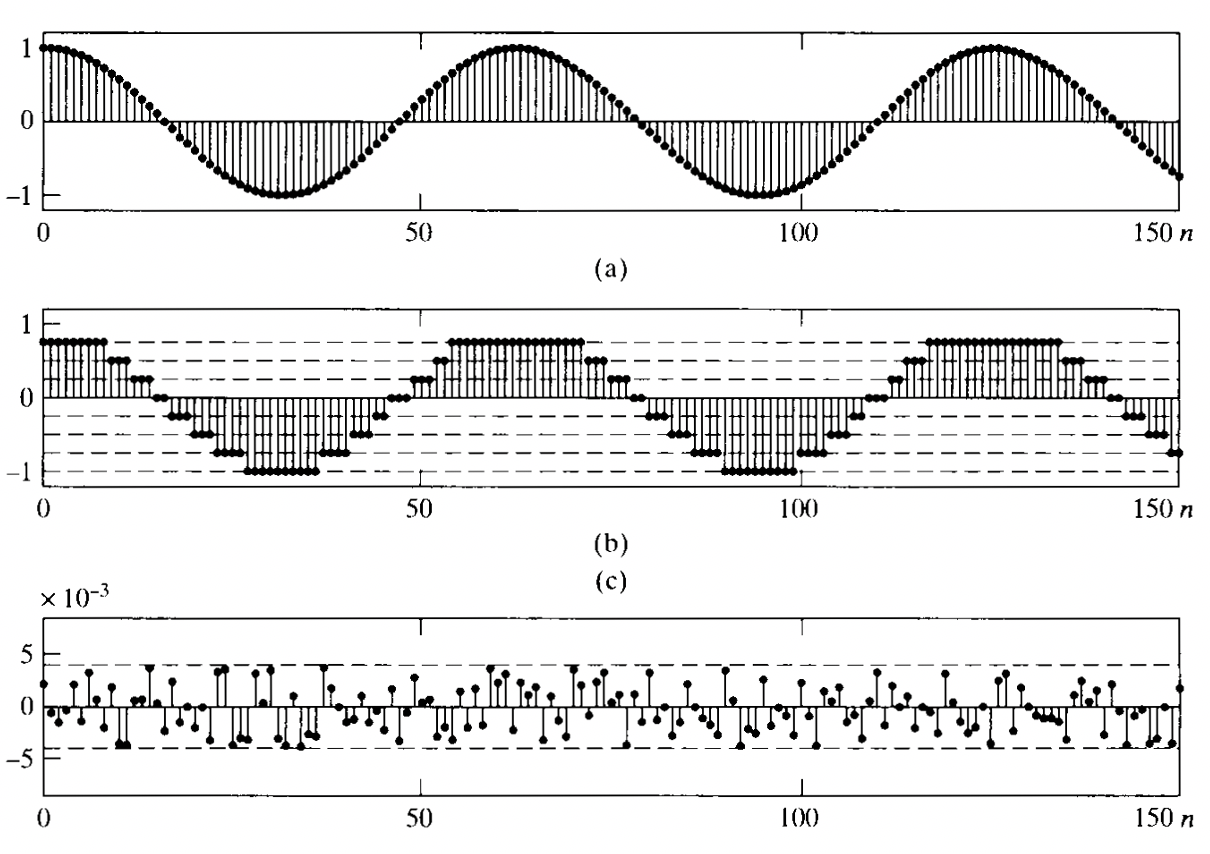
\includegraphics[width = 0.6\textwidth]{images/1.2.1}
    \caption{Sampling and quantisation}
 \end{figure}
 \textit{We focus on the signals of one independent variable!}
 
\subsection{Deterministic and Stochastic Signals}
 \begin{itemize}
    \item \textbf{Deterministic}: a signal that \textbf{can be predicted} exactly (an analytical formulation exists). 
     \begin{itemize}
        \item Example: $x(t) = \sin(2\pi t)$
      \end{itemize}
      
    \item \textbf{Stochastic}: a signal that \textbf{cannot be predicted} exactly before it has “occurred”; any signal that conveys information to us when we observe it. 
      \begin{itemize}
        \item Example: Thermal noise across a resistor, EEG traces, etc.
      \end{itemize}
      
    \item We can often meaningfully describe the statistical properties of stochastic signals by building a model of their generation (stochastic processes).
 \end{itemize}
\textit{We will mainly deal with deterministic signals in this course!}

\subsection{Periodic Signals}
 \begin{itemize}
    \item A periodic continuous-time signal $x(t)$ has the property that there is a positive value of $T$ for which $x(t) = x(t+T)$ for all values of $t$ (similar definition for discrete-time signals).
    
    \item A periodic signal has the property that it is unchanged by a time shift of $T$, we will say that $x(t)$ is periodic with period $T$. (\textsc{Fig.3})
 \end{itemize}
 \begin{figure}[H]\centering
    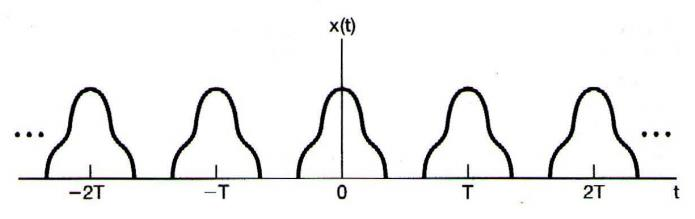
\includegraphics[width = 0.6\textwidth]{images/1.5}
    \caption{A periodic signal with period $T$}
 \end{figure}

\subsection{Signal Energy and Power}
For a continuous-time signal $x(t)$ for $t_1 \leq t \leq t_2$ and for a discrete-time signal $x[n]$ for $n_1 \leq n \leq n_2$, energy and power can be represented as follows:
\[ \text{Energy(continuous time)} = \int_{t_1}^{t_2} \lvert x(t) \rvert^2 \ dt \]
\[ \text{Power(continuous  time)} = \frac{1}{t_2 - t_1} \ \int_{t_1}^{t_2} \ \lvert x(t) \rvert^2 \ dt \]
\[ \text{Energy(discrete time)} = \sum_{n_1}^{n_2} \ \lvert x[n] \rvert ^2 \]
\[ \text{Power(discrete time)} = \frac{1}{n_2 - n_1} \sum_{n_1}^{n_2} \ \lvert x[n] \rvert ^2 \]

\begin{tcolorbox}[title= Electrical circuit analogy, breakable]
 %\underline{\textsc{Derivation}}\\
  We get the conclusion above from the calculation for electrical power and energy.
  Let $v(t)$ and $i(t)$ represent the voltage and current across the resistor of resistance $R$. 
 \begin{itemize}
  \item The instantaneous power across the resistor is the product $v(t)i(t)$, which is proportional to $v^2(t)$.
  \item The total energy \[ \int_{t_1}^{t_2} \ \frac{1}{R} \ v^2(t) \ dt \] 
  \item The average power \[ \frac{1}{t_2 - t_1} \ \int_{t_1}^{t_2} \ \frac{1}{R} \ v^2(t) \ dt \]
  \end{itemize}
  Similar properties can be applied to any continuous-time signals and discrete-time signals.
\end{tcolorbox}
  
\begin{itemize}
 \item Often, the signals are directly related to physical quantities capturing power and energy in a physical form.
 \item These properties are important characteristics of signals, even if in some cases do not reflect physical energy or power.
 %\item Therefore, we extend the above definition of energy and power to any continuous-time signal as well as discrete-time signal (including the case of complex signals)
\end{itemize}

\subsubsection{Energy and Power of a Generic Signal}
%We extend the previous definition to any continuous-time signal $x(t)$ for $t_1 \leq t \leq t_2$ and and discrete-time signal $x[n]$ for $n_1 \leq n \leq n_2$, as follows:
%\[ Energy(continuous \ time) = \int_{t_1}^{t_2} \lvert x(t) \rvert^2 \ dt \]
%\[ Power(continuous \ time) = \frac{1}{t_2 - t_1} \ \int_{t_1}^{t_2} \ \lvert x[n] \rvert^2 \ dt \]
%\[ Energy(discrete \ time) = \sum_{n_1}^{n_2} \ \lvert x[n] \rvert ^2 \]
%\[ Power(discrete \ time) = \frac{1}{n_2 - n_1} \sum_{n_1}^{n_2} \ \lvert x[n] \rvert ^2 \]
Extend the range to: $-\infty<t<+\infty$ or $-\infty<n<+\infty$ 
\begin{itemize}
 \item In continuous time:
  \[ \text{Energy}= \int_{-\infty}^{+\infty} \ \lvert x(t) \rvert^2 \ dt \]
  \[ \text{Power}= \lim_{T \to \infty} \ \frac{1}{2T} \ \int_{-T}^{T} \ \lvert x(t) \rvert^2 \ dt \]
 \item In discrete time:
  \[ \text{Energy}= \sum_{-\infty}^{+\infty} \ \lvert x[n] \rvert^2 \]
  \[ \text{Power}=\lim_{N \to +\infty} \ \frac{1}{2N+1} \ \sum_{-N}^{N} \ \lvert x[n] \rvert^2 \]
\end{itemize}
\textit{We will use the mathematical definitions above, regardless of the direct physical meaning of each term!}